\documentclass[border=10pt]{standalone}

\usepackage{tikz}
\usepackage{tikzsymbols}
\usetikzlibrary{calc,patterns,shapes.geometric}

\def\centerarc[#1](#2)(#3:#4:#5){\draw[#1] ($(#2)+({#5*cos(#3)},{#5*sin(#3)})$) arc (#3:#4:#5);}

\begin{document}
	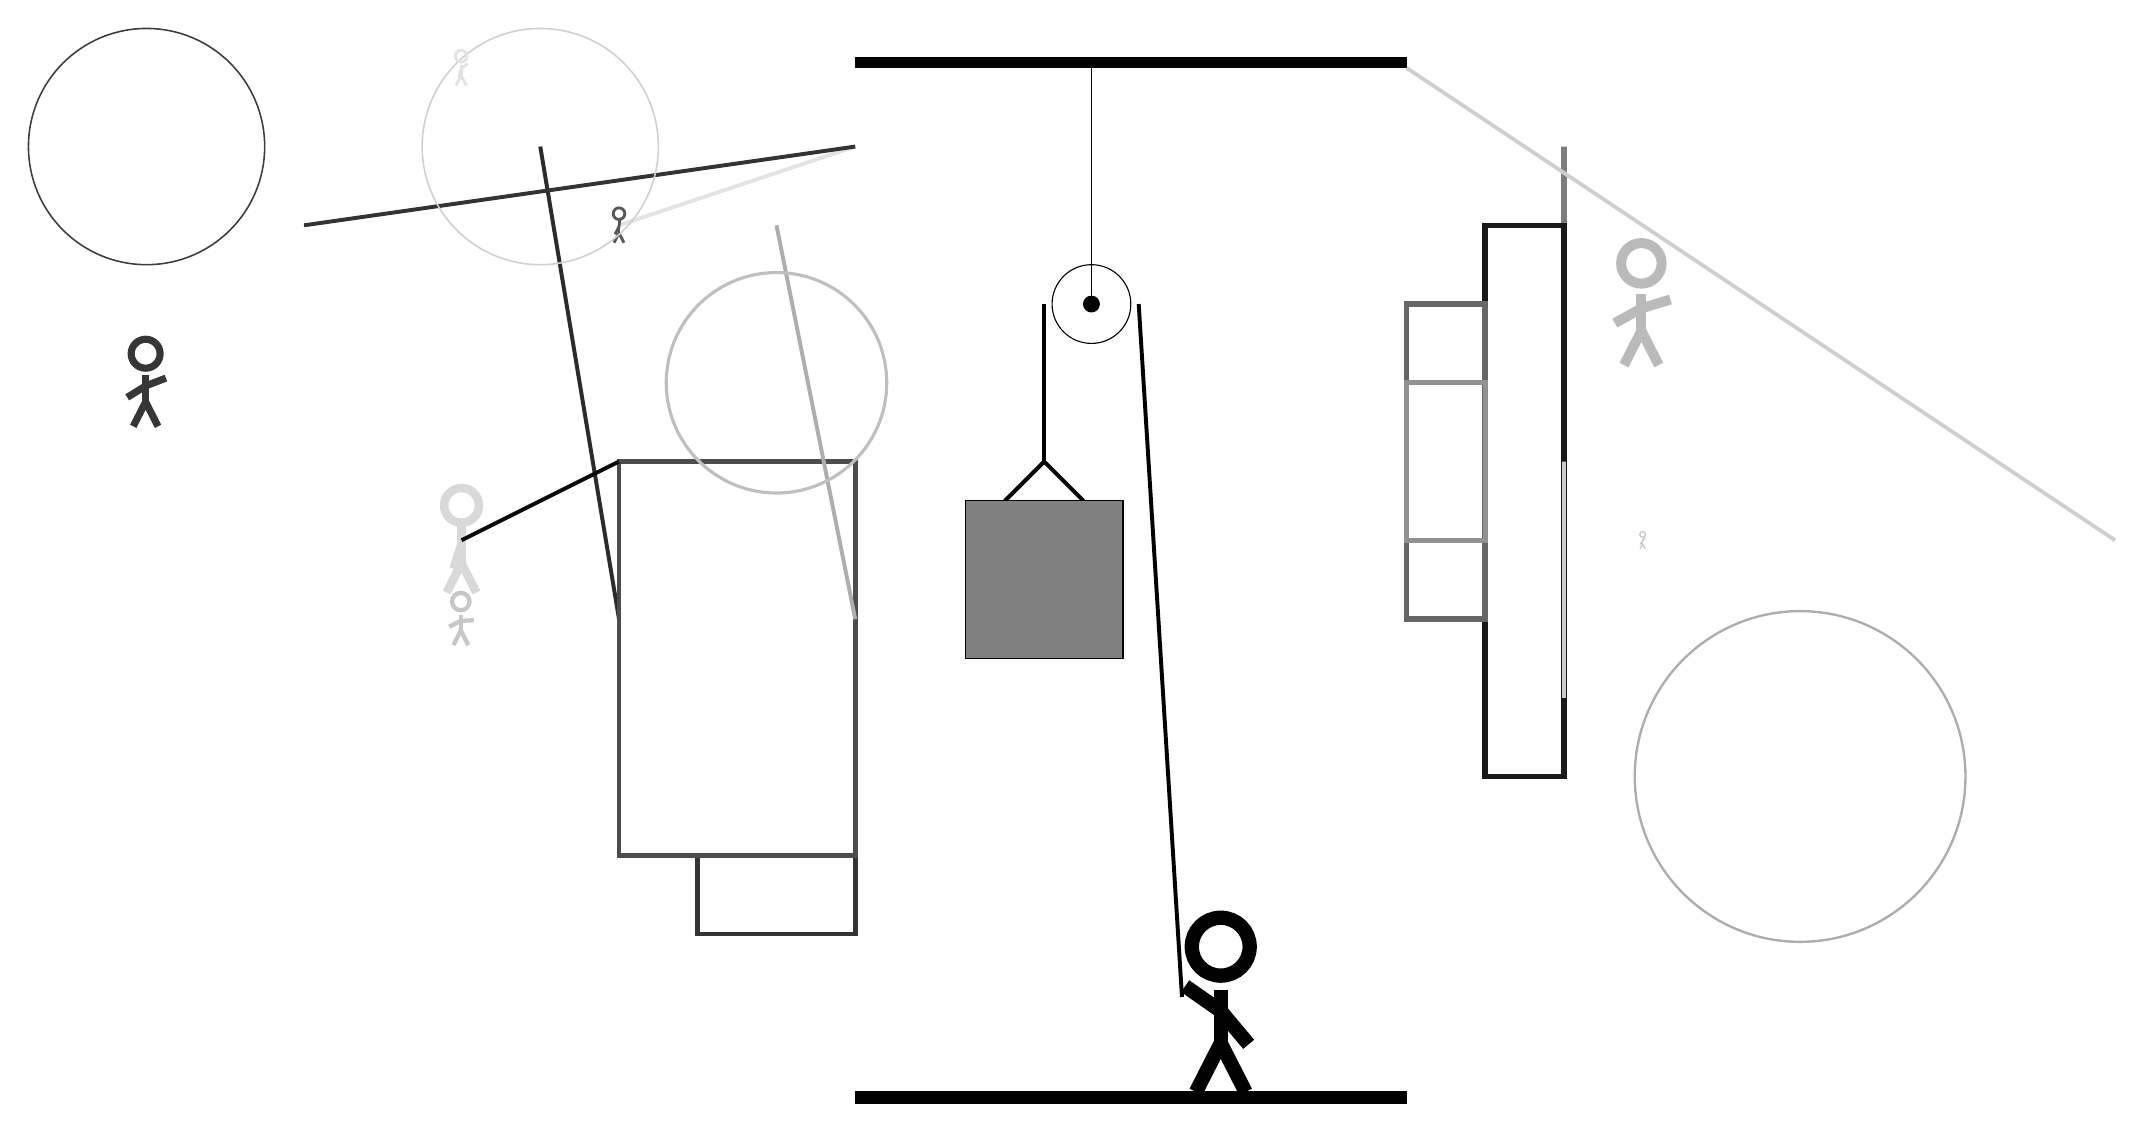
\begin{tikzpicture}
		%%%%% START %%%%%
		
		\draw[fill=black] (-2, 10) rectangle (5, 10.125);
		
		\draw (1, 7) circle (0.5);
		\draw[fill=black] (1, 7) circle (0.1);
		\draw (1, 10) -- (1, 7);
		
		\draw[line width=0.5mm] (-0.1, 4.5) -- (0.4, 5.0) -- (0.9, 4.5);
		\draw[fill=black!50] (-0.6, 4.5) rectangle (1.4, 2.5);
		
		\draw[line width=0.5mm] (0.4, 7) -- (0.4, 5.0);
		\centerarc[line width=0.5mm](1, 7)(0:180:0.6);
		\draw[line width=0.5mm](1.6, 7) -- (2.15, -1.8);
		
		\draw[line width=0.6mm, color=black!80] (-2, -1) rectangle (-4, 0);
		
		\draw[line width=0.5mm, color=black!83](-6, 9) -- (-5, 3);
		\draw [line width=0.3mm, color=black!32](10, 1) circle (2.1);
		\draw[line width=0.7mm, color=black!52] (5, 6) rectangle (5, 3);
		\draw[line width=0.7mm, color=black!51] (7, 9) rectangle (7, 3);
		\draw[line width=0.6mm, color=black!70] (-2, 0) rectangle (-5, 5);
		
		\node[line width=0.5mm, color=black!22] at (-7, 3) {\Strichmaxerl[3][27][3]};
		\draw[line width=0.5mm, color=black!11](-5, 8) -- (-2, 9);
		\node[line width=0.4mm, color=black!27] at (8, 7) {\Strichmaxerl[7][29][17]};
		\node[line width=0.7mm, color=black!79] at (-11, 6) {\Strichmaxerl[5][32][21]};
		\draw[line width=0.7mm, color=black!90] (7, 1) rectangle (6, 8);
		\draw[line width=0.6mm, color=black!20] (7, 2) rectangle (7, 5);
		\draw[line width=0.5mm, color=black!32](-3, 8) -- (-2, 3);
		
		\node[line width=0.5mm, color=black!15] at (-7, 4) {\Strichmaxerl[6][72][90]};
		\node[line width=0.2mm, color=black!66] at (-5, 8) {\Strichmaxerl[2][63][83]};
		\draw[line width=0.7mm, color=black!60] (6, 3) rectangle (5, 7);
		\draw[line width=0.6mm, color=black!43] (5, 6) rectangle (6, 4);
		
		\draw[line width=0.5mm, color=black!96](-5, 5) -- (-7, 4);
		\draw[line width=0.5mm, color=black!19](5, 10) -- (14, 4);
		
		\draw[line width=0.5mm, color=black!80](-2, 9) -- (-9, 8);
		\draw [line width=0.2mm, color=black!76](-11, 9) circle (1.5);
		\node[line width=0.4mm, color=black!21] at (8, 4) {\Strichmaxerl[1][56][53]};
		\draw [line width=0.4mm, color=black!25](-3, 6) circle (1.4);
		\draw [line width=0.2mm, color=black!19](-6, 9) circle (1.5);
		\node[line width=0.6mm, color=black!11] at (-7, 10) {\Strichmaxerl[2][75][40]};
		
		
		\node at (2.6, -1.9) {\Strichmaxerl[10][-35][-50]};
		
		\draw[fill=black] (-2, -3) rectangle (5, -3.15);
		
		%%%%% END %%%%%
	\end{tikzpicture}
\end{document}